
\section{Yorug`likning qutublanishi}



\begin{enumerate}

\item Quyidagi 2 ta fikrning qaysi biri to‘g‘ri?
\begin{itemize}
    \item[a)] $\vec{E}$ vektorining amplitudasi barcha tebranish tekisligida birday bo‘lsa, uni tabiiy yorug‘lik deyiladi.
    \item[b)] $\vec{E}$ vektorining tebranishlari hamma vaqt faqat birgina tekislikda sodir bo‘lsa, uni yassi qutblangan yorug‘lik deyiladi.
\end{itemize}
\begin{enumerate}[label=\Alph*)]
\item faqat a.
\item faqat b.
\item ikkalasi ham to‘g‘ri.
\item ikkalasi ham noto‘g‘ri.
\end{enumerate}

\item Turmalin yoki boshqa qutblovchi kristallardan tabiiy nur o‘tganda, uning intensivlik bo‘yicha qanday maksimal qismi qutblangan nur bo‘lib o‘tadi?
\begin{enumerate}[label=\Alph*)]
\item 0,75.
\item 0,25.
\item 0,5.
\item 0,125.
\end{enumerate}

\item Agar turmalin plastinasiga tushayotgan tabiiy yorug‘lik intensivligi $I_0$ bo‘lsa, undan o‘tayotgan yorug‘lik intensivligi $I$ nimaga teng?
\begin{enumerate}[label=\Alph*)]
\item $I_0$.
\item $I_0/8$.
\item $I_0/4$.
\item $I_0/2$.
\end{enumerate}

\item Analizator yorug‘lik intensivligini 1,5625 marta kamaytiradi. Polarizator va analizatorning optik o‘qlari orasidagi burchakni aniqlang.

\begin{center}
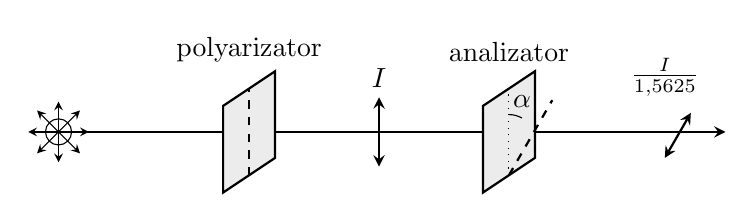
\begin{tikzpicture}[scale=1.1, >=stealth]
  % Markaziy o'q (nur yo'nalishi)
  \draw[thick, ->] (-2.5,0) -- (5.5,0);

  % Tabiiy yorug'lik ramzi (aylana ichida ko'p yo'nalishli strelkalar)
  \node at (-2.2, 0) [circle, draw, minimum size=0.3cm] (c) {};
  \foreach \a in {0, 45, 90, 135} {
    \draw[<->, thin] (-2.2,0) +(\a:0.35) -- +(\a+180:0.35);
  }

  % Polarizator
  \draw[thick, fill=gray!15] (-0.3,-0.7) -- (0.3,-0.3) -- (0.3,0.7) -- (-0.3,0.3) -- cycle;
  \draw[dashed, thick] (0, -0.5) -- (0, 0.5);
  \node[above] at (0, 0.7) {polyarizator};

  % Oraliq qutblangan nur (vertikal)
  \draw[<->, thick] (1.5, -0.4) -- (1.5, 0.4);
  \node[above] at (1.5, 0.4) {$I$};

  % Analizator
  \draw[thick, fill=gray!15] (2.7,-0.7) -- (3.3,-0.3) -- (3.3,0.7) -- (2.7,0.3) -- cycle;
  % Vertikal chiziq va qiya optik o'q
  \draw[dotted] (3.0, -0.5) -- (3.0, 0.5);
  \draw[dashed, thick] (3.0, -0.5) -- +(60:1.0);
  \draw (3.0, 0.2) arc (90:60:0.3);
  \node at (3.15, 0.35) {$\alpha$};
  \node[above] at (3.0, 0.7) {analizator};

  % Chiqishdagi nur (qiya)
  \draw[<->, thick] (4.8, -0.3) -- +(60:0.6);
  \node[above] at (4.8, 0.3) {$\frac{I}{1,5625}$};
\end{tikzpicture}
\end{center}

\begin{enumerate}[label=\Alph*)]
\item $30^\circ$.
\item $45^\circ$.
\item $60^\circ$.
\item $37^\circ$.
\end{enumerate}

\item Yorug‘lik to‘lqini bo‘ylama to‘lqinmi, ko‘ndalang to‘lqinmi?
\begin{enumerate}[label=\Alph*)]
\item ham ko‘ndalang, ham bo‘ylama.
\item bo‘ylama.
\item ko‘ndalang.
\item to‘lqin uzunligiga bog‘liq.
\end{enumerate}

\item Yorug‘lik to‘lqinining bo‘ylama yoki ko‘ndalang ekanligini qaysi hodisa yordamida aniqlash mumkin?
\begin{enumerate}[label=\Alph*)]
\item dispersiya.
\item qutblanish.
\item interferensiya.
\item difraksiya.
\end{enumerate}

\item Quyida keltirilgan hodisalardan qaysi biri yorug‘lik to‘lqinining ko‘ndalangligini tasdiqlaydi?
\begin{enumerate}[label=\Alph*)]
\item yorug‘likning qutblanishi.
\item difraksiya.
\item interferensiya.
\item dispersiya.
\end{enumerate}

\item Quyidagi to‘lqinlardan qaysilari qutblanish xossasiga ega?
1) tovush to‘lqini; 2) yorug‘lik to‘lqini; 3) radioto‘lqinlar.
\begin{enumerate}[label=\Alph*)]
\item faqat 1.
\item faqat 2.
\item hammasi.
\item 2 va 3.
\end{enumerate}

\item Quyida sanalgan to‘lqinlardan qaysilari ko‘ndalang to‘lqinlar turiga kiradi?
1) suv betidagi to‘lqinlar; 2) gazdagi tovush to‘lqinlari; 3) yorug‘lik to‘lqinlari; 4) radioto‘lqinlar; 5) suyuqlikdagi ultratovush to‘lqinlari.
\begin{enumerate}[label=\Alph*)]
\item 2, 4, 5.
\item 1, 2, 3.
\item 4, 5.
\item 1, 3, 4.
\end{enumerate}

\item Quyida sanab o‘tilgan to‘lqinlarning qaysilari ko‘ndalang?
1) tovush; 2) suv sirtidagi to‘lqinlar; 3) elektromagnit to‘lqinlar; 4) ikki uchi mahkamlangan sim tebranishidagi to‘lqinlar; 5) siqilayotgan va kengayayotgan prujinadagi to‘lqinlar.
\begin{enumerate}[label=\Alph*)]
\item 1, 2, 3.
\item 2, 3, 5.
\item 4, 5.
\item 2, 3, 4.
\end{enumerate}

\item Quyida sanalgan to‘lqinlardan qaysilari bo‘ylama to‘lqinlar turiga kiradi?
1) suv sirtidagi to‘lqinlar; 2) gazlardagi tovush to‘lqinlari; 3) radioto‘lqinlar; 4) suyuqlikdagi ultratovush to‘lqinlari; 5) yorug‘lik to‘lqinlari.
\begin{enumerate}[label=\Alph*)]
\item 1, 2.
\item 2, 4.
\item 2, 3.
\item 3, 4.
\end{enumerate}

\item Keltirilgan hodisalardan qaysilari yorug‘likning to‘lqin nazariyasi asosida tushuntiriladi?
1) interferensiya; 2) difraksiya; 3) fotoeffekt; 4) yorug‘likning qutblanishi.
\begin{enumerate}[label=\Alph*)]
\item 1, 2, 3.
\item 2, 3.
\item hammasi.
\item 1, 2, 4.
\end{enumerate}

\end{enumerate}




\begin{table}[!ht]
\centering
\begin{tabular}{|c|c|c|c|c|c|c|c|c|c|c|}
\hline
1c & 2c & 3d & 4d & 5c & 6b & 7a & 8d & 9d & 10d & 11b \\ \hline
12d & & & & & & & & & & \\ \hline
\end{tabular}
\end{table}